% A simple neuralnet with one hidden layer.

\begin{figure}[htbp]
\renewcommand{\familydefault}{\sfdefault}\normalfont
\centering

\def\layersep{2.0cm}

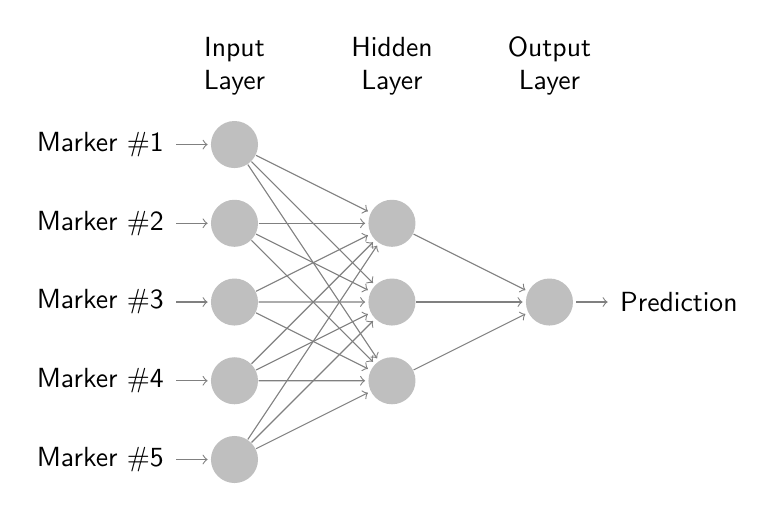
\begin{tikzpicture}[shorten >=1pt, ->, draw=black!50, node distance=\layersep]
    \tikzstyle{every pin edge}=[<-, shorten <=1pt]

    \tikzstyle{neuron}=[circle, fill=black!25,minimum size=17pt, inner sep=0pt]
    \tikzstyle{input neuron}=[neuron];
    \tikzstyle{output neuron}=[neuron];
    \tikzstyle{hidden neuron}=[neuron];

    \tikzstyle{annot}=[text width=4em, text centered]

    \foreach \name / \y in {1,...,5}
        \node[input neuron, pin=left:Marker \#\y] (I-\name) at (0,-\y) {};

    \foreach \name / \y in {1,...,3}
        \path[yshift=-1cm]
            node[hidden neuron] (H-\name) at (\layersep,-\y cm) {};

    \node[output neuron, pin={[pin edge={->}]right:Prediction}, right of=H-2] (0) {};

    \foreach \source in {1,...,5}
        \foreach \dest in {1,...,3}
            \path (I-\source) edge (H-\dest);

    \foreach \source in {1,...,3}
        \path (H-\source) edge (0);

    \node[annot, above of=I-1, node distance=1cm] (il) {Input Layer};
    \node[annot, right of=il] (hl) {Hidden Layer};
    \node[annot, right of=hl] {Output Layer};
\end{tikzpicture}

    \caption{A multi-layer perceptron neural network with a single hidden layer. 
             Many input calls are mapped into the hidden layer of neurons. For genomic
             prediction, the input layer consists of one neuron per marker and the output
             consists of a single neuron which combines the information from the final
             hidden layer to predict a phenotype or BLUP. Because this network has only
             a single hidden layer, it would not be considered a deep network.}

\label{fig:simplenet}
\end{figure}
